\documentclass[a4paper,twocolumn,11pt]{article}
\usepackage[utf8]{inputenc}
\usepackage[MeX]{polski}
\usepackage[top=3cm, bottom=3cm, left=2.5cm, right=2.5cm]{geometry}
\usepackage[breaklinks=true]{hyperref}
\usepackage{amsfonts}
\usepackage{amsthm}
\usepackage{ragged2e}
\usepackage{tikz}
\usetikzlibrary{calc,shapes,shapes.multipart,arrows,chains}
\usepackage{tikz-uml}
\usepackage[explicit]{titlesec}
\usepackage{caption}

% ;;;;;;;;; colors ;;;;;;;;;;;;

\definecolor{Board}{RGB}{60,145,143}
\definecolor{DoubleWordBonus}{RGB}{239,174,154}
\definecolor{DoubleLetterBonus}{RGB}{141,201,240}
\definecolor{TripleLetterBonus}{RGB}{54,156,219}
\definecolor{Tile}{RGB}{247,225,190}
\definecolor{UniGreen}{RGB}{0,100,200}

% ;;;;;;;;; theorems ;;;;;;;;;;;;

\theoremstyle{definition}
\newtheorem{theorem}{Twierdzenie}
\newtheorem{definition}{Definicja}
\newtheorem{pro}{Dowód}

% ;;;;;;;;; macros ;;;;;;;;;;;;

\newlength{\mysize}
\newcommand{\mycfs}[1]{\setlength{\mysize}{#1pt}%
  \fontsize{\mysize}{1.2\mysize}\selectfont}
\newcommand{\mycfsb}[1]{\bfseries \mycfs{#1}}
\renewcommand{\captionfont}{\centering \mycfs{10}}
\renewcommand{\captionlabelfont}{\mycfsb{10}}

% ;;;;;;;;; headers ;;;;;;;;;;;;

\titleformat{\section}[runin]{\bfseries}{}{0pt}{\thesection. #1}[]
\titleformat{name=\section,numberless}[runin]{\bfseries}{}{0pt}{#1}[]
\titleformat{\subsection}[runin]{\bfseries}{}{0pt}{\thesubsection. #1}[]
\titlespacing*{\section} {0pt}{6pt}{2.3ex plus .2ex}
\titlespacing*{\subsection} {0pt}{3pt}{1.5ex plus .2ex}

% ;;;;;;;;; spacing ;;;;;;;;;;;;

\setlength\parindent{0.4cm}
\setlength{\columnsep}{0.8cm}

% ;;;;;;;;;;;;;;;;;;;;;;;;;;;;;;;;

\title{{\mycfsb{14} Zaawansowana sztuczna inteligencja do Scrabble.} \\ {\mycfsb{14} Podstawy teoretyczne i~opis implementacji algorytmu.}}
\author{{\mycfs{12} Jakub Turek} \\ {\mycfs{11} Wydział Elektroniki i~Technik Informacyjnych} \\ {\mycfs{11} J.Turek@stud.elka.pw.edu.pl}}
\date{}

\begin{document}

\vspace{1.5cm}

\maketitle

\section*{Streszczenie}

\emph{Celem artykułu jest opisanie zbioru koncepcji, które posłużą do implementacji algorytmu sztucznej inteligencji grającego w~grę Scrabble w~języku polskim. Artykuł prezentuje zbiór teoretycznych informacji o~optymalnej strategii gry w~Scrabble. Ponadto zostały w~nim przedstawione elementy algorytmów zastosowanych w~aplikacjach Maven oraz Quackle. Autor wskazuje ich potencjalne słabe punkty i~sposoby usprawnienia, a~także prezentuje wyniki implementacji proponowanych poprawek.}

\section{Wstęp}

Scrabble to ,,gra słowna polegająca na układaniu na określonej planszy wyrazów z~losowanych liter''. \cite{scrabble_definition} Jest to bardzo ogólna definicja, którą należy uściślić. Scrabble jest grą przeznaczoną dla 2-4 osób. Akcesoriami do gry są: kwadratowa plansza o~stałym rozmiarze $15 \times 15$, torebka wypełniona płytkami, na których nadrukowane są litery oraz ich wartości punktowe, a~także stojaki, na których gracze umieszczają płytki, którymi w~danej chwili dysponują.

Gra rozgrywana jest w~turach. Zadaniem graczy jest układanie wyrazów na planszy w~taki sposób, aby tworzyły one poprawne słowa w~języku, w~którym prowadzona jest rozgrywka, w~układzie krzyżówkowym. Układ krzyżówkowy został przedstawiony na rysunkach \ref{fig:crossword_first} oraz \ref{fig:crossword_second}:

\begin{description}
 \item [Rysunek \ref{fig:crossword_first}] Pokazuje sytuację początkową obrazującą pewien moment rozgrywki.
 \item [Rysunek \ref{fig:crossword_second}] Pokazuje poprawny ruch zawodnika, który powoduje powstanie więcej niż jednego słowa. Wszystkie wyrazy utworzone przez jeden ruch muszą być poprawne. W~podanym przykładzie słowa ,,za'' i~,,masz'' są poprawne.
\end{description}

\begin{figure}[ht!]
	\begin{center}
			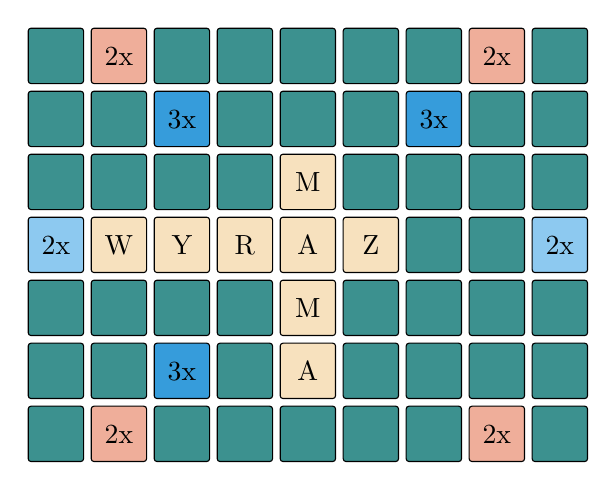
\begin{tikzpicture}
			\tikzstyle{every node}=[draw, shape=rectangle, rounded corners = 1pt, minimum width = 20pt, minimum height = 20pt, align=center, text height = 7pt];
			\node [fill=Board] at (-0.8, 0) {};
			\node [fill=DoubleWordBonus] at (0, 0) {2x};
			\node [fill=Board] at (0.8, 0) {};
			\node [fill=Board] at (1.6, 0) {};
			\node [fill=Board] at (2.4, 0) {};
			\node [fill=Board] at (3.2, 0) {};
			\node [fill=Board] at (4.0, 0) {};
			\node [fill=DoubleWordBonus] at (4.8, 0) {2x};
			\node [fill=Board] at (5.6, 0) {};
			\node [fill=Board] at (-.8, -.8) {};
			\node [fill=Board] at (0, -.8) {};
			\node [fill=TripleLetterBonus] at (0.8, -.8) {3x};
			\node [fill=Board] at (1.6, -.8) {};
			\node [fill=Board] at (2.4, -.8) {};
			\node [fill=Board] at (3.2, -.8) {};
			\node [fill=TripleLetterBonus] at (4.0, -.8) {3x};
			\node [fill=Board] at (4.8, -.8) {};
			\node [fill=Board] at (5.6, -.8) {};
			\node [fill=Board] at (-.8, -1.6) {};
			\node [fill=Board] at (0, -1.6) {};
			\node [fill=Board] at (0.8, -1.6) {};
			\node [fill=Board] at (1.6, -1.6) {};
			\node [fill=Tile] at (2.4, -1.6) {M};
			\node [fill=Board] at (3.2, -1.6) {};
			\node [fill=Board] at (4.0, -1.6) {};
			\node [fill=Board] at (4.8, -1.6) {};
			\node [fill=Board] at (5.6, -1.6) {};
			\node [fill=DoubleLetterBonus] at (-.8, -2.4) {2x};
			\node [fill=Tile] at (0, -2.4) {W};
			\node [fill=Tile] at (.8, -2.4) {Y};
			\node [fill=Tile] at (1.6, -2.4) {R};
			\node [fill=Tile] at (2.4, -2.4) {A};
			\node [fill=Tile] at (3.2, -2.4) {Z};
			\node [fill=Board] at (4.0, -2.4) {};
			\node [fill=Board] at (4.8, -2.4) {};
			\node [fill=DoubleLetterBonus] at (5.6, -2.4) {2x};
			\node [fill=Board] at (-.8, -3.2) {};
			\node [fill=Board] at (0, -3.2) {};
			\node [fill=Board] at (0.8, -3.2) {};
			\node [fill=Board] at (1.6, -3.2) {};
			\node [fill=Tile] at (2.4, -3.2) {M};
			\node [fill=Board] at (3.2, -3.2) {};
			\node [fill=Board] at (4.0, -3.2) {};
			\node [fill=Board] at (4.8, -3.2) {};
			\node [fill=Board] at (5.6, -3.2) {};
			\node [fill=Board] at (-.8, -4.0) {};
			\node [fill=Board] at (0, -4.0) {};
			\node [fill=TripleLetterBonus] at (0.8, -4.0) {3x};
			\node [fill=Board] at (1.6, -4.0) {};
			\node [fill=Tile] at (2.4, -4.0) {A};
			\node [fill=Board] at (3.2, -4.0) {};
			\node [fill=Board] at (4.0, -4.0) {};
			\node [fill=Board] at (4.8, -4.0) {};
			\node [fill=Board] at (5.6, -4.0) {};
			\node [fill=Board] at (-.8, -4.8) {};
			\node [fill=DoubleWordBonus] at (0, -4.8) {2x};
			\node [fill=Board] at (0.8, -4.8) {};
			\node [fill=Board] at (1.6, -4.8) {};
			\node [fill=Board] at (2.4, -4.8) {};
			\node [fill=Board] at (3.2, -4.8) {};
			\node [fill=Board] at (4.0, -4.8) {};
			\node [fill=DoubleWordBonus] at (4.8, -4.8) {2x};
			\node [fill=Board] at (5.6, -4.8) {};
		\end{tikzpicture}
		\caption{Fragment planszy. Gracze ułożyli kolejno słowa: ,,wyraz'' oraz ,,mama''.}
		\label{fig:crossword_first}
	\end{center}
\end{figure}

\begin{figure}[ht!]
	\begin{center}
			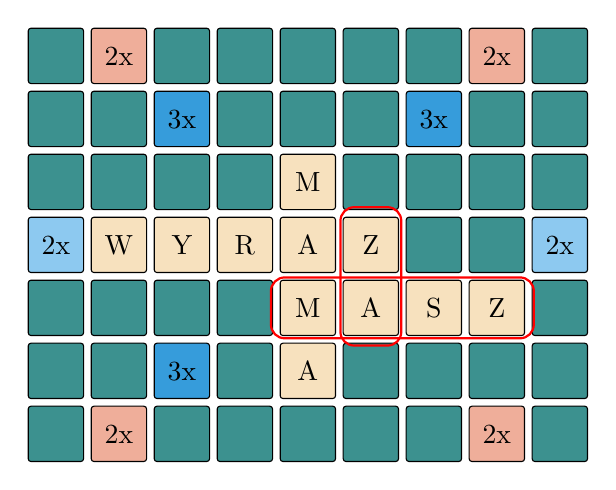
\begin{tikzpicture}
			\tikzstyle{every node}=[draw, shape=rectangle, rounded corners = 1pt, minimum width = 20pt, minimum height = 20pt, align=center, text height = 7pt];
			\node [fill=Board] at (-0.8, 0) {};
			\node [fill=DoubleWordBonus] at (0, 0) {2x};
			\node [fill=Board] at (0.8, 0) {};
			\node [fill=Board] at (1.6, 0) {};
			\node [fill=Board] at (2.4, 0) {};
			\node [fill=Board] at (3.2, 0) {};
			\node [fill=Board] at (4.0, 0) {};
			\node [fill=DoubleWordBonus] at (4.8, 0) {2x};
			\node [fill=Board] at (5.6, 0) {};
			\node [fill=Board] at (-.8, -.8) {};
			\node [fill=Board] at (0, -.8) {};
			\node [fill=TripleLetterBonus] at (0.8, -.8) {3x};
			\node [fill=Board] at (1.6, -.8) {};
			\node [fill=Board] at (2.4, -.8) {};
			\node [fill=Board] at (3.2, -.8) {};
			\node [fill=TripleLetterBonus] at (4.0, -.8) {3x};
			\node [fill=Board] at (4.8, -.8) {};
			\node [fill=Board] at (5.6, -.8) {};
			\node [fill=Board] at (-.8, -1.6) {};
			\node [fill=Board] at (0, -1.6) {};
			\node [fill=Board] at (0.8, -1.6) {};
			\node [fill=Board] at (1.6, -1.6) {};
			\node [fill=Tile] at (2.4, -1.6) {M};
			\node [fill=Board] at (3.2, -1.6) {};
			\node [fill=Board] at (4.0, -1.6) {};
			\node [fill=Board] at (4.8, -1.6) {};
			\node [fill=Board] at (5.6, -1.6) {};
			\node [fill=DoubleLetterBonus] at (-.8, -2.4) {2x};
			\node [fill=Tile] at (0, -2.4) {W};
			\node [fill=Tile] at (.8, -2.4) {Y};
			\node [fill=Tile] at (1.6, -2.4) {R};
			\node [fill=Tile] at (2.4, -2.4) {A};
			\node [fill=Tile] at (3.2, -2.4) {Z};
			\node [fill=Board] at (4.0, -2.4) {};
			\node [fill=Board] at (4.8, -2.4) {};
			\node [fill=DoubleLetterBonus] at (5.6, -2.4) {2x};
			\node [fill=Board] at (-.8, -3.2) {};
			\node [fill=Board] at (0, -3.2) {};
			\node [fill=Board] at (0.8, -3.2) {};
			\node [fill=Board] at (1.6, -3.2) {};
			\node [fill=Tile] at (2.4, -3.2) {M};
			\node [fill=Tile] at (3.2, -3.2) {A};
			\node [fill=Tile] at (4.0, -3.2) {S};
			\node [fill=Tile] at (4.8, -3.2) {Z};
			\node [fill=Board] at (5.6, -3.2) {};
			\node [fill=Board] at (-.8, -4.0) {};
			\node [fill=Board] at (0, -4.0) {};
			\node [fill=TripleLetterBonus] at (0.8, -4.0) {3x};
			\node [fill=Board] at (1.6, -4.0) {};
			\node [fill=Tile] at (2.4, -4.0) {A};
			\node [fill=Board] at (3.2, -4.0) {};
			\node [fill=Board] at (4.0, -4.0) {};
			\node [fill=Board] at (4.8, -4.0) {};
			\node [fill=Board] at (5.6, -4.0) {};
			\node [fill=Board] at (-.8, -4.8) {};
			\node [fill=DoubleWordBonus] at (0, -4.8) {2x};
			\node [fill=Board] at (0.8, -4.8) {};
			\node [fill=Board] at (1.6, -4.8) {};
			\node [fill=Board] at (2.4, -4.8) {};
			\node [fill=Board] at (3.2, -4.8) {};
			\node [fill=Board] at (4.0, -4.8) {};
			\node [fill=DoubleWordBonus] at (4.8, -4.8) {2x};
			\node [fill=Board] at (5.6, -4.8) {};
			\node [draw, thick, shape = rectangle, rounded corners = 5pt, color = red, fill = none, minimum height = 22 pt, minimum width = 95 pt] at (3.6, -3.2) {};
			\node [draw, thick, shape = rectangle, rounded corners = 5pt, color = red, fill = none, minimum width = 22 pt, minimum height = 50 pt] at (3.2, -2.8) {};
		\end{tikzpicture}
		\caption{Fragment planszy. Ruch przez dołożenie liter A, S, Z tworzy dwa wyrazy w~układzie krzyżówkowym.}
		\label{fig:crossword_second}
	\end{center}
\end{figure}

W~trakcie jednego ruchu zawodnik może układać płytki tylko w~jednym kierunku (pionowo lub poziomo). Utworzony przez zawodnika wyraz musi być spójny, to znaczy, że wszystkie płytki muszą przylegać do siebie bezpośrednio lub poprzez płytki już istniejące na planszy. Wymagane jest, aby tworzone słowo przylegało do przynajmniej jednej płytki, która jest już umieszczona na planszy (nie dotyczy to pierwszego ruchu).

Punktacja za dane zagranie jest obliczana jako suma punktów za wszystkie płytki, które wchodzą w~skład utworzonych wyrazów (a~więc również tych, które przed zagraniem znajdowały się na planszy), z~uwzględnieniem niewykorzystanych premii wynikających z~pozycji płytki na planszy:

\begin{description}
 \item [Premia literowa] podwaja lub potraja wartość danej płytki.
 \item [Premia słowna] podwaja lub potraja wartość całego wyrazu.
\end{description}

\section{Strategia optymalna}

Kluczowym zagadnieniem podczas implementacji algorytmu sztucznej inteligencji do gier planszowych (w~tym Scrabble) jest zbadanie istnienia strategii optymalnej.

\begin{theorem}
	Istnieje optymalna strategia gry w~Scrabble.
	\label{thm:optimal_strategy_existence}
\end{theorem}

Aby dowieść twierdzenie \ref{thm:optimal_strategy_existence}~należy uprzednio zdefiniować przestrzeń stanów w~Scrabble.

\begin{definition}
	Stan rozgrywki po danej turze opisują jednoznacznie rozmieszczenie klocków na planszy $P$~oraz zagranie $Z$. Przejście między stanami determinuje zmiana $(\Delta P, \Delta Z)$.
	\label{def:scrabble_state_space}
\end{definition}

Dysponując definicją \ref{def:scrabble_state_space}~można dowieść twierdzenie \ref{thm:optimal_strategy_existence}. Ilustrację dla dowodu \ref{pro:optimal_strategy_existence}~przedstawia rysunek \ref{fig:state_space}.

\begin{pro}
	Dla ułatwienia analiza rozgrywki zostanie przeprowadzona wychodząc od stanu końcowego. Nie wpływa to na ogólność dowodu. Dla dowolnej rozgrywki prawdziwe jest twierdzenie, że do stanu końcowego można wejść tylko na skończoną liczbę sposobów, które reprezentują legalne zagrania. Przeprowadzając rozumowanie iteracyjne możliwe jest przejście do stanu początkowego. Należy zauważyć, że w~każdej iteracji analizowana liczba wejść do stanu jest zawsze skończona, ponieważ skończona jest liczba kombinacji, na które można wylosować litery oraz liczba zagrań legalnych dla danej kombinacji liter. Podobne rozumowanie można przeprowadzić dla każdego stanu końcowego budując skończone drzewo przestrzeni stanów. Skoro drzewo przestrzeni stanów jest skończone, można na podstawie jego znajomości w~każdym zagraniu wyznaczyć ruch, który maksymalizuje prawdopodobieństwo wygranej.
	\label{pro:optimal_strategy_existence}
\end{pro}

\begin{figure}[ht!]
	\begin{center}
			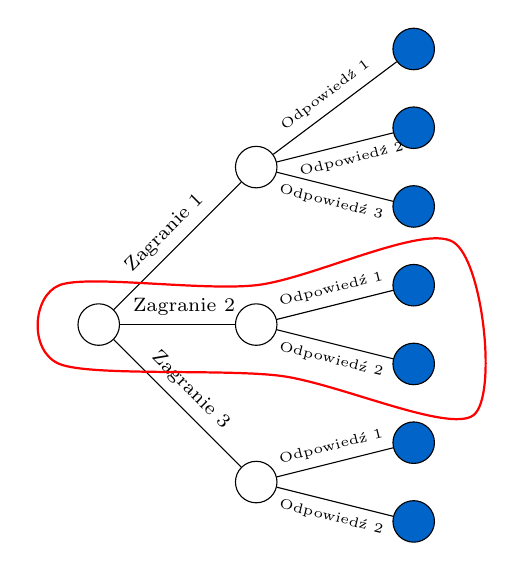
\begin{tikzpicture}
				\tikzstyle{state} = [draw, shape=circle, minimum width=15pt, minimum height=15pt]
				\node (s0) [state] at (0,0) {};
				\node (s1) [state] at (2,2) {};
				\node (s2) [state] at (2,0) {};
				\node (s3) [state] at (2, -2) {};
				\node (s4) [state, fill=UniGreen] at (4,3.5) {};
				\node (s5) [state, fill=UniGreen] at (4,2.5) {};
				\node (s6) [state, fill=UniGreen] at (4,1.5) {};
				\node (s7) [state, fill=UniGreen] at (4,0.5) {};
				\node (s8) [state, fill=UniGreen] at (4,-0.5) {};
				\node (s9) [state, fill=UniGreen] at (4,-1.5) {};
				\node (s10) [state, fill=UniGreen] at (4,-2.5) {};
				\draw (s0) -- node[above, sloped, font=\scriptsize] {Zagranie 1} (s1);
				\draw (s0) -- node[above, sloped, font=\scriptsize, near end, xshift=-8pt] {Zagranie 2} (s2);
				\draw (s0) -- node[above, sloped, font=\scriptsize] {Zagranie 3} (s3);
				\draw (s1) -- node[above, sloped, font=\tiny] {Odpowiedź 1} (s4);
				\draw (s1) -- node[xshift=-6pt, below, near end, sloped, font=\tiny] {Odpowiedź 2} (s5);
				\draw (s1) -- node[below, sloped, font=\tiny] {Odpowiedź 3} (s6);
				\draw (s2) -- node[above, sloped, font=\tiny] {Odpowiedź 1} (s7);
				\draw (s2) -- node[below, sloped, font=\tiny] {Odpowiedź 2} (s8);
				\draw (s3) -- node[above, sloped, font=\tiny] {Odpowiedź 1} (s9);
				\draw (s3) -- node[below, sloped, font=\tiny] {Odpowiedź 2} (s10);
				\draw [red, thick] plot [smooth cycle] coordinates {(-0.5, -0.5) (-0.5, 0.5) (2, 0.5) (4.5, 1.05) (4.76, -1.15) (2.3, -0.65)};
			\end{tikzpicture}
			\caption{Ilustracja dowodu istnienia strategii optymalnej. Stany końcowe oznaczono kolorem niebieskim.}
			\label{fig:state_space}
	\end{center}
\end{figure}

Zostało udowodnione, że deterministyczna wersja Scrabble dla dwóch graczy należy do problemów klasy \emph{PSPACE-Complete}. \cite{deterministic_scrabble} Klasa \emph{PSPACE-Complete} jest najbardziej obszerną klasą problemów wielomianowych. Każdy problem należący do przestrzeni problemów wielomianowych można przekształcić, w~wielomianowym czasie, do problemu klasy \emph{PSPACE-Complete}.

\section{Strategia zależna od fazy gry}

Niestety, w~praktyce wykorzystywanie strategii optymalnej nie jest możliwe. Dla rozgrywki końcowej 7~klocków przeciwko 7~klockom średnia ilość gałęzi w~drzewie przestrzeni stanów wynosi 200. Kolejnym problemem jest głębokość drzewa, która może sięgać czternastu poziomów (gdy gracze wykładają klocki pojedynczo) lub więcej (dochodzi możliwość pasowania). Wartości te są zbyt duże aby stosować pełny algorytm typu $\alpha - \beta$, a~odnoszą się wyłącznie do sytuacji, w~której posiadamy pełną informację o~rozgrywce (to znaczy znane są klocki przeciwnika). Na pozostałych etapach rozgrywki analiza przestrzeni stanów nie jest opcją. Wynika z~tego, że algorytm sztucznej inteligencji do Scrabble musi zmieniać strategię rozgrywki w~zależności od etapu gry.

Wyróżnia się cztery zasadnicze fazy rozgrywki: \cite{sheppard_maven}

\begin{description}
	\item[Opening Play\footnotemark] \footnotetext{Opening Play, w~skrócie OP. W~dalszej części artykułu dla określenia faz rozgrywki stosowane będą wyłącznie nazwy skrótowe, a~więc OP, MG, PEG oraz EG.} faza otwarcia. Dotyczy wyłącznie pierwszego zagrania, a~więc kiedy na planszy nie znajduje się jeszcze żaden klocek.
	\item[Mid Game] faza śródgry. Rozpoczyna się po otwarciu, a~kończy wraz z~rozpoczęciem fazy PEG.
	\item[Pre-End Game] faza przedkońcowa rozgrywki. Rozpoczyna się w~momencie, w~którym rozgrywka może zakończyć się w~dwóch turach, a~więc kiedy w~worku pozostaje siedem lub mniej klocków. Kończy się wraz z~rozpoczęciem fazy EG.
	\item[End Game] faza zakończenia. Rozpoczyna się, gdy w~worku nie ma już klocków i~trwa aż do końca gry. Charakteryzuje się tym, że w~trakcie jej trwania zawodnicy dysponują pełną informacją o~grze, a~więc również o~literach posiadanych przez przeciwnika.
\end{description}

Wykonywany algorytm będzie różny w~zależności od fazy rozgrywki. Podczas implementacji takiego rozwiązania warto wykorzystać wzorzec projektowy Strategia. Strategia to wzorzec, który ,,definiuje rodzinę algorytmów, pakuje je jako osobne klasy i~powoduje, że są one w pełni wymienne. Zastosowanie strategii pozwala na to, aby zmiany w~implementacji przetwarzania były całkowicie niezależne od strony klienta, który z nich korzysta''. \cite{strategy_pattern_definition} Wzorzec strategii dostosowany do opisywanej dziedziny problemu został schematycznie przedstawiony na rysunku \ref{fig:strategy_pattern}.

\begin{figure}[ht!]
	\centering
	\scalebox{0.7}{
		\begin{tikzpicture}
			\tikzumlset{fill class=white!100}
			\umlclass[type=interface,x=0,y=4]{ScrabbleAI}{\# phase : GamePhase}{+ move() : void \\ \# pickStrategy() : IMoveStrategy} 
			\umlclass[type=interface,x=0,y=0]{IMoveStrategy}{}{+ move() : void} 
			\umlclass[x=-3, y=-3]{FirstPlayStrategy}{}{+ move() : void}
			\umlclass[x=0, y=-6]{MidGameStrategy}{}{+ move() : void}
			\umlclass[x=3, y=-3]{EndGameStrategy}{}{+ move() : void}
			\umluniassoc{ScrabbleAI}{IMoveStrategy}
			\umlimpl{IMoveStrategy}{FirstPlayStrategy}
			\umlimpl{IMoveStrategy}{MidGameStrategy}
			\umlimpl{IMoveStrategy}{EndGameStrategy}
		\end{tikzpicture}
	}
	\caption{Przykład użycia wzorca projektowego Strategia w~kontekście implementacji algorytmu.}
	\label{fig:strategy_pattern}
\end{figure}

\section{Opening Play}

Celem fazy OP jest wybranie najwyżej punktowanego zagrania. W~algorytmie Quackle wybór ten jest dokonywany poprzez przeszukiwanie słownika pod kątem posiadanych liter. Wynik punktowy uzyskany za zagranie jest obliczany dynamicznie. 

Wyszukiwanie najlepszego otwarcia może być zoptymalizowane czasowo. Wykorzystując znajomość słownika można przeprowadzić analizę najlepszych otwarć dla wszystkich możliwych kombinacji klocków. Każdej kombinacji liter można przypisać prostą funkcję skrótu, która sortuje te litery alfabetycznie. Po wstępnej analizie słownika można przygotować mapę, która każdej funkcji skrótu przyporządkuje najlepsze zagranie oraz jego wartość punktową. Dzięki temu możliwe jest wykonanie pierwszego zagrania w~czasie jednostkowym\footnote{Przy założeniu, że wśród liter początkowych nie znajdują się blanki.}.

\section{Mid Game}

W~fazie MG w~aplikacji Quackle wykorzystywany jest algorytm z~heurystyczną funkcją oszacowania oraz symulacją dwóch zagrań ,,w~przód''. Schemat tego algorytmu został przedstawiony na rysunku \ref{fig:mid_game_algorithm}.~\cite{quackle_algorithm}

\begin{figure}[ht!]
	\centering
	\scalebox{0.55}{
		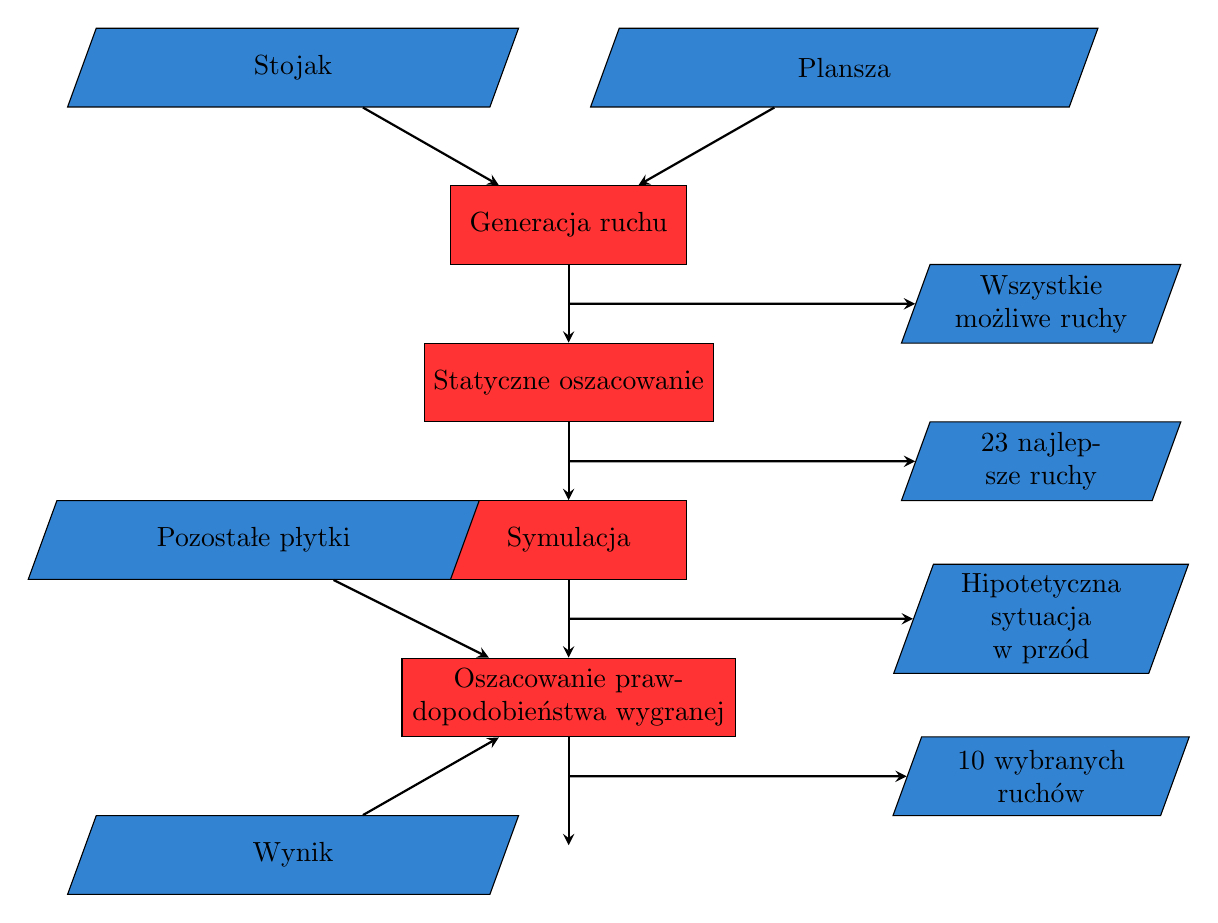
\begin{tikzpicture}[node distance=2cm]
			\noindent
			\tikzstyle{io} = [trapezium, trapezium left angle=70, trapezium right angle=110, minimum width=2cm, minimum height=1cm, text centered, draw=black, fill=UniGreen!80, text width=2.5cm]
			\tikzstyle{process} = [rectangle, minimum width=3cm, minimum height=1cm, text centered, draw=black, fill=red!80]
			\tikzstyle{arrow} = [thick,->,>=stealth]
					
			\node (rack) [io] {Stojak};
			\node (board) [io, right of=rack, xshift=5cm] {Plansza};
			\coordinate (rackboard) at ($(rack)!0.5!(board)$);
			\node (movegen) [process, below of= rackboard] {Generacja ruchu};
			\node (staticeval) [process, below of=movegen] {Statyczne oszacowanie};
			\coordinate (movegenstaticeval) at ($(movegen)!0.5!(staticeval)$);
			\node (possmoves) [io, right of=movegenstaticeval, xshift=4cm] {Wszystkie możliwe ruchy};
			\node (simulation) [process, below of=staticeval] {Symulacja};
			\node (bestmoves) [io, below of=possmoves] {23 najlepsze ruchy};
			\node (hypsequences) [io, below of=bestmoves] {Hipotetyczna sytuacja w~przód};
			\node (winpercestimation) [process, below of=simulation, text width=4cm] {Oszacowanie prawdopodobieństwa wygranej};
			\node (end) [process, draw=none, fill=none, below of=winpercestimation, minimum height=1mm] { };
			\coordinate (staticevalsimulation) at ($(staticeval)!0.5!(simulation)$);
			\node (tilesleft) [io, left of=winpercestimation,xshift=-2cm,yshift=2cm] {Pozostałe płytki};
			\node (score) [io, left of=winpercestimation,xshift=-1.5cm,yshift=-2cm] {Wynik};
			\coordinate (winpercestimationend) at ($(winpercestimation)!0.5!(end)$);
			\node (chosenmoves) [io, below of=hypsequences] {10 wybranych ruchów};
			\draw [arrow] (movegen) -- (staticeval);
			\draw [arrow] (staticeval) -- (simulation);
			\draw [arrow] (simulation) -- (winpercestimation);
			\draw [arrow] (rack) -- (movegen);
			\draw [arrow] (board) -- (movegen);
			\draw [arrow] (winpercestimation) -- (end);
			\draw [arrow] (tilesleft) -- (winpercestimation);
			\draw [arrow] (score) -- (winpercestimation);
			\draw [arrow] ($(movegen)!0.5!(staticeval)$) -- (possmoves);
			\draw [arrow] ($(staticeval)!0.5!(simulation)$) -- (bestmoves);
			\draw [arrow] ($(simulation)!0.5!(winpercestimation)$) -- (hypsequences);
			\draw [arrow] ($(winpercestimation)!0.5!(end)$) -- (chosenmoves);
		\end{tikzpicture}
	}
	\caption{Schemat algorytmu dla fazy MG.}
	\label{fig:mid_game_algorithm}
\end{figure}

Algorytm składa się z~czterech kroków:

\begin{enumerate}
	\item Na podstawie stanu planszy i~dostępnych klocków generowane są wszystkie możliwości ruchu.
	\item Dla każdej możliwości ruchu obliczana jest funkcja oszacowania. Ruchy są sortowane względem malejącej wartości funkcji oszacowania. Lista ruchów jest skracana do najlepszych 23 pozycji.
	\item Dla każdego z~pozostałych ruchów wykonywana jest symulacja stanu rozgrywki na dwa kroki w~przód.
	\item Dla każdego rezultatu oszacowania, biorąc pod uwagę liczbę płytek pozostałych do końca rozgrywki, obliczane jest prawdopodobieństwo wygranej. W~rezultacie powstaje lista 10 ruchów o~największym oszacowanym prawdopodobieństwie wygranej.
\end{enumerate}

Na potrzeby artykułu pominięte zostanie omówienie fazy generacji ruchu. Jej wynikiem jest lista wszystkich poprawnych ruchów dla określonej kombinacji liter i~ułożenia klocków na planszy.

\subsection{Statyczne oszacowanie}

Do statycznego oszacowania wykorzystywana jest funkcja celu postaci $F(x) = P(x) + LV(x)$, gdzie $F(x)$ to wartość oszacowania dla zagrania $x$, $P(x)$ to wartość punktowa tego zagrania, a~$LV(x)$ to współczynnik \emph{leave value} dla klocków pozostałych po zagraniu.

\begin{definition}
	\emph{Leave value} to funkcja, która zestawowi klocków pozostałych po zagraniu przypisuje wartość punktową odzwierciedlającą ,,perspektywiczność'' pod kątem wysoko punktowanych zagrań w~przyszłości. Funkcja przyjmuje wartości należące do zbioru $\mathbb{R}$ liczb rzeczywistych.
\end{definition}

Przykładowo jeśli płytki pozostałe po ułożeniu czteroliterowego wyrazu to \textbf{Ą}, \textbf{Ź}~oraz \textbf{Ń}, wtedy ich wartość \emph{leave value} będzie ujemna, gdyż prawdopodobieństwo siedmioliterowego zagrania w~kolejnym ruchu jest bardzo niskie. Wartości funkcji \emph{leave value} wyznaczane są na podstawie bazy danych wcześniejszych gier, którą można zbudować wykorzystując zapisy partii z~turniejów.

Statyczne oszacowanie przeprowadza się dla wszystkich dozwolonych ruchów wyznaczonych na etapie generacji. Do kolejnego etapu wybierane są 23 ruchy z~najwyższą wartością funkcji celu.

\subsection{Symulacja}

W~fazie symulacji dla każdego z~pozostałych 23 ruchów szacuje się jaki może być ich skutek na dwa zagrania w~przód. Symulacja przeprowadzana jest według poniższego algorytmu:

\begin{enumerate}
	\item Gracz $G_{1}$ wykonuje zagranie $P_{1}$.
	\item Ze zbioru pozostałych płytek wybierana jest losowa zawartość stojaka gracza $G_{2}$.
	\item Generowane są wszystkie możliwości ruchu dla gracza $G_{2}$.
	\item Gracz $G_{2}$ wykonuje zagranie $P_{2}$ z~najwyższą wartością statycznego oszacowania.
	\item Gracz $G_{1}$ uzupełnia płytki. 
	\item Generowane są wszystkie możliwości ruchu dla gracza $G_{1}$.
	\item Gracz $G_{1}$ wykonuje zagranie $P_{3}$ z~najwyższą wartością statycznego oszacowania.
	\item Dla zagrania $P_{1}$ obliczana jest wartość symulacji $PV_{1}$. Jest to liczba punktów $G_{1}$ po zagraniu $P_{3}$ pomniejszona o~liczbę punktów $G_{2}$ po zagraniu $P_{2}$.
	\item Wartość $PV_{1}$ jest powiększana o~\emph{leave value} płytek gracza $G_{1}$ po zagraniu $P_{3}$.
\end{enumerate}

\subsection{Szacowanie prawdopodobieństwa wygranej}

Dla każdego z~23 wyników symulacji szacowane jest następnie prawdopodobieństwo wygranej. Prawdopodobieństwo wygranej jest funkcją $W: PV, TR \rightarrow [0;1]$, gdzie $PV$ jest wartością zagrania wyznaczoną w trakcie symulacji, a~$TR$ jest liczbą klocków pozostałych do wykorzystania w~partii. 

Wartości funkcji $W$, podobnie jak wartości funkcji celu dla fazy statycznego oszacowania, są wyznaczane na podstawie bazy danych gier. W~wyniku etapu oszacowania prawdopodobieństwa wygranej pozostawiane jest 10 zagrań o~największym prawdopodobieństwie wygranej.

\subsection{Usprawnienia fazy mid-game}

Na etapie symulacji pomijane są dwa istotne aspekty rozgrywki:

\begin{itemize}
	\item Losowanie zawartości stojaka przeciwnika odbywa się z~rozkładem jednostajnym. Obserwując poprzedni ruch przeciwnika można lepiej przybliżyć ten rozkład.
	\item Gracze korzystają z~\emph{łowienia} korzystnych wyrazów.
\end{itemize}

Jeżeli w~poprzednim ruchu przeciwnik ułożył na planszy słowo \textbf{RADO} można wnioskować, że nie posiadał on liter \textbf{I} oraz \textbf{U}. W~przeciwnym razie utworzyłby wyżej punktowane słowa - \textbf{RADIO} lub \textbf{URODA}. Korzystając z~tej obserwacji możemy wylosować $\frac{3}{7}$ zawartości stojaka przeciwnika ze zbioru pozostałych klocków z~pominięciem liter \textbf{U} oraz \textbf{I}. 

\begin{definition}
	\emph{Łowienie} w~grze Scrabble to umyślny brak wykorzystania większości klocków do wykonania zagrania ze względu na duże prawdopodobieństwo wylosowania układu pozwalającego na wysoko punktowane zagranie w~kolejnym ruchu.
\end{definition}

Niestety, w~praktyce trudno określić kryteria, które pozwalają rozpoznać \emph{łowienie} przeciwnika. Umiarkowanie dobrym kryterium jest analiza ilości liter użytych do poprzedniego zagrania. Jeżeli przeciwnik wykorzystał tylko jedną literę bardzo prawdopodobne jest, że próbował \emph{złowić} dobrą kombinację liter. Aby przeciwdziałać \emph{łowieniu} należy wybrać specjalną estymatę zawartości stojaka przeciwnika na etapie symulacji. Dzięki temu symulacja preferować będzie zagrania blokujące \emph{hot-spoty}, czyli otwarte punkty planszy umożliwiające wysoko punktowaną rozgrywkę.

Kolejnym usprawnieniem algorytmu może być wprowadzenie rozróżnienia na zagrania ofensywne oraz defensywne. Etap oszacowania prawdopodobieństwa wygranej bazuje na nieprecyzyjnych informacjach wejściowych. Zasymulowana pozycja ,,w~przyszłości'' może być nieadekwatna do rzeczywistości, na przykład gdy zostało pominięte możliwe \emph{bingo} przeciwnika. Wprowadzając podział zagrań na defensywne i~ofensywne możliwe jest wprowadzenie dodatkowego elementu algorytmu rozważającego opłacalność zagrania otwierającego planszę. Do rozważania opłacalności można wykorzystać sieć neuronową.

Podział zagrań na defensywne i~ofensywne można przeprowadzić na podstawie wielu kryteriów. Pod uwagę można brać między innymi liczbę wykorzystanych podczas zagrania klocków, które znajdowały się na planszy przed rozegraniem. Innym przykładem takiego kryterium jest ilość nowych premii otwartych w~wyniku zagrania.

\section{End Game}

Algorytm operujący w~fazie EG dysponuje pełną informacją o~grze, gdyż wiadomo jakimi literami dysponuje przeciwnik. W~tych warunkach naturalne jest wykorzystanie przeszukiwania przestrzeni stanów algorytmem typu $\alpha - \beta$. Niestety, nawet w~końcowych etapach rozgrywki przestrzeń stanów jest zbyt duża i~zbyt głęboka aby wykonać takie przeszukiwane. Niezbędne jest wyznaczenie ograniczeń.

Do wyznaczania ograniczeń można wykorzystać programowanie dynamiczne. Na potrzeby oszacowania przyjęte zostanie założenie, że sytuacja na planszy jest statyczna i~wartość możliwych do uzyskania zagrań zależy jedynie od stanu planszy i~zawartości stojaka, a~nie superpozycji kolejnych zagrań obu graczy. Zakładając, że partia zakończy się w~$N$~ruchach można ograniczyć przeszukiwaną przestrzeń tylko do $N$ poziomów. Każdemu zagraniu zostanie przypisana jego szacowana wartość w~postaci $F_{N}(x) = P_{N}(x) + LV_{N-1}$. $P_{N}$ oznacza liczbę punktów uzyskanych za zagranie, a~$LV_{N-1}$ to oszacowanie wartości pozostałych po zagraniu płytek przy założeniu, że do końca rozgrywki pozostało $N - 1$ tur.

Przykład oszacowania dla fazy EG:

\begin{enumerate}
	\item Gracz 1~($G_{1}$) zakończy grę w~8~ruchach. Wtedy gracz 2~($G_{2}$) rozegra 7~ruchów. Powstaje ścieżka do przetworzenia algorytmem minimax.
	\item $G_{2}$ zakończy grę w~7 ruchach. $G_{1}$ rozegra wtedy 7 ruchów. Jeżeli ta ścieżka będzie lepsza dla $G_{2}$, $G{2}$ wybierze właśnie ją.
	\item $G_{1}$ będzie miał okazję do poprawy jeżeli zakończy grę w~7~ruchach...
\end{enumerate}

Algorytm ten jest kontynuowany do momentu, gdy żaden z~graczy nie może się poprawić.

Analiza przestrzeni stanów może być dalej usprawniana. Nie zawsze istnieje bowiem jedna optymalna ścieżka zagrania dla przeciwnika. Przykładowo, gdy może on zagrać słowo \textbf{ALE} w~dwóch różnych pozycjach (za 25 i~28 punktów odpowiednio) korzyść z~zablokowania drugiej na rzecz pierwszej pozycji wynosi tylko trzy punkty. Spostrzeżenie to można zawrzeć w~algorytmie przez wprowadzenie dwóch progów oszacowania: optymistycznego i~pesymistycznego. Niestety, algorytm minimax nie wspiera przedziałów. Do przeszukiwania przestrzeni stanów należy zatem wykorzystać inny algorytm. Przykładem przeszukiwania wspierającego przedziały jest algorytm $B^{*}$. \cite{bstar}

\section{Pre-end Game}

W~fazie PEG obliczenia wykonywane przez algorytm dla fazy MG pozostaną poprawne. Pod uwagę należy wziąć również scenariusz końca gry, gdyż wraz z~rozpoczęciem fazy PEG możliwe jest zakończenie rozgrywki w~dwóch turach. Rozwiązaniem jest wykorzystywanie hybrydowego podejścia, które najpierw wyznacza najkorzystniejsze ruchy algorytmem dla fazy MG, a~potem dokonuje dla nich ograniczonego przeszukiwania przestrzeni stanów.

\section{Wyniki testów}

Na potrzeby testowania usprawnień algorytmów przedstawionych w~artykule zostały wykonane dwie implementacje sztucznej inteligencji do Scrabble. Jedna, nazywana dalej algorytmem referencyjnym, bazuje bezpośrednio na specyfikacji aplikacji Quackle. \cite{quackle_algorithm} Druga, tak zwany algorytm zmodyfikowany, nanosi do algorytmu referencyjnego wszystkie modyfikacje opisane w~artykule. Oba algorytmy rozegrały przeciwko sobie 1523 partie. Podsumowanie wyników zostało zamieszczone w~tabeli~\ref{tab:test_results}.

\begin{figure}[ht!]
	\centering
	\scalebox{0.95}{
		\begin{tabular}{|l|c|c|}
			\hline
			& 	Algorytm		&	Algorytm		\\
			& 	zmodyfikowany 	& 	referencyjny 	\\
			\hline
			Wygrane 		& 	987				& 	536				\\
			\hline
			\% wygranych	&   \textbf{64,8\%} & 	35,2\%			\\
			\hline
		\end{tabular}
	}
	\caption{Wyniki testów modyfikacji algorytmu referencyjnego.}
	\label{tab:test_results}
\end{figure}

Rozkład procentowy wygranych znacząco odbiega od rozkładu $50\% - 50\%$, którego można byłoby oczekiwać dla równorzędnych przeciwników. Na podstawie przedstawionej próby można wnioskować, że modyfikacje wprowadzone do algorytmu przyczyniły się do zwiększenia jego skuteczności.

Ze względu na brak odpowiedniej klasy przeciwników algorytm nie został należycie przetestowany przeciwko ludziom. Okazało się, że przewaga, którą daje znajomość całego słownika jest zbyt duża, aby gracze-amatorzy mogli wygrać chociaż jedną partię z~algorytmem. W~dotychczasowych testach zmodyfikowany algorytm odniósł $100\%$ zwycięstw.

\section{Podsumowanie}

Artykuł prezentuje informacje, które mogą posłużyć do implementacji zaawansowanego algorytmu sztucznej inteligencji grającego w~Scrabble. Artykuł przedstawia podstawy teoretyczne niezbędne do jego implementacji. Ponadto opisuje szczegółowo  strategie, które mogą być stosowane na różnym stopniu zaawansowania rozgrywki. 

Artykuł koncentruje się na wskazaniu słabych ogniw algorytmów dla poszczególnych etapów rozgrywki. Autor prezentuje modyfikacje, które należy wprowadzić celem eliminacji omawianych wad. Zaprezentowane w~artykule wyniki testów pozwalają sądzić, że wprowadzone modyfikacje pozytywnie wpływają na skuteczność całego algorytmu. 

Dalszym kierunkiem rozwoju algorytmu może być badanie sposobu na wykrycie próby \emph{złowienia} dobrych liter przez przeciwnika. Testy algorytmu referencyjnego wskazują, że wiele przegranych wynika z~powszechnego wykorzystywania \emph{łowienia} przez zawodników klasy mistrzowskiej. Zaproponowany w~artykule sposób wykrywania tego typu zagrań nie jest wyczerpujący i~może być przedmiotem dalszych usprawnień. Dalszemu badaniu może podlegać również efektywność wprowadzonych modyfikacji dla innych języków rozgrywki.

\begin{thebibliography}{9}
	\small
	\bibitem{scrabble_definition} 
		\emph{Wielki słownik ortograficzny PWN}, pod red. Edwarda Polańskiego, Wyd. 3 popr. i~uzup., Warszawa, Wydawnictwo Naukowe PWN, 2012, ISBN 978-83-01-16405-8.
	\bibitem{scrabble_word_rules}
		\emph{Zasady dopuszczalności słów} [online], Polska Federacja Scrabble [dostęp: 25 kwietnia 2014], Dostępny w~Internecie: \href{http://www.pfs.org.pl/zds.php}{\nolinkurl{<http://www.pfs.org.pl/zds.php>}}.
	\bibitem{deterministic_scrabble} M. Lampis, V. Mitsou, K. Sołtys, \emph{Scrabble is PSPACE-Complete}, 2012.
	\bibitem{sheppard_maven} B. Sheppard, \emph{World-championship-caliber Scrabble}, ,,Artificial Intelligence'', vol. 134, p. 241-275, 2002.
	\bibitem{strategy_pattern_definition} E.~Freeman, B.~Bates, K.~Sierra, \emph{Rusz głową! Wzorce projektowe}, Wyd. 2, Gliwice, Wydawnictwo Helion, 2011, ISBN 978-83-246-2803-2, strona 56.
	\bibitem{quackle_algorithm}
		Jason Katz-Brown, John O'Laughlin, \emph{How Quackle Plays Scrabble} [online], Quackle [dostęp: 25 kwietnia 2014], Dostępny w~Internecie: \href{http://people.csail.mit.edu/jasonkb/quackle/doc/how_quackle_plays_scrabble.html}{\nolinkurl{<http://people.csail.mit.edu/jasonkb/quackle/doc/how\_quackle\_plays\_scrabble.html>}}.
	\bibitem{bstar} H.~J.~Berliner, C.~McConnell, \emph{$B^{*}$ Probability Based Search}, Carnegie Mellon University, 1995.
\end{thebibliography}

\end{document}
